\documentclass[lang=cn,10pt]{elegantbook}
\setcounter{tocdepth}{3}
% 本文档命令
\usepackage{array}
\usepackage{physics}
\renewcommand{\i}{\mathrm{i}}
\newcommand{\ccr}[1]{\makecell{{\color{#1}\rule{1cm}{1cm}}}}
\everymath{\displaystyle}%行间公式
\author{光电2班\quad 夏明宇\quad 21201128}
\title{数学物理方法期中作业}
\subtitle{复变函数总结}
\date{\zhtoday}
\institute{杭州电子科技大学\quad 理学院}
\bioinfo{教师}{童常青}
\setcounter{tocdepth}{3}
% 修改标题页的橙色带
 \definecolor{customcolor}{RGB}{197, 232, 198}
 \colorlet{coverlinecolor}{customcolor}
\logo{School of Science.pdf}
\cover{chaptercover.png}
\begin{document}
\maketitle
\frontmatter
\mainmatter
\newpage
\begin{spacing}{2.4}
\chapter*{前言}
这学期为学习了《数学物理方法》，该课程总共分为两部分，分别是《复变函数》与《数学物理方程》.本文档为《复变函数》知识点的一个个人整理与归纳。


在学习《复变函数》的过程中，我本人比较感兴趣的，是留数定理部分。这一部分仿佛是在一个被称作“复球面”的幻想世界，在这里，被C-R选中的函数将被授予“全纯”，导引解析之力。而我则扮演一位名为“积分”的神秘角色，在复合闭路中邂逅性质各异、展开独特的级数们，和他们一起击败奇点，找回失散的留数——同时，逐步发掘“三大变换”的真相。


总的来说，和以往的思维不同，平时计算实数范围内的广义积分，通常都是采用一些比较基本的方法，而对于一些较为复杂的积分，普通的方法就可能难以解决；这时，如果采用留数定理，寻找被积函数的奇点，并计算留数，就可以轻松计算出该积分，无论从难度上、还是准确性上，较普通方法都超越了许多。也是因为这令人耳目一新的计算积分的方法，使我对此很感兴趣。下面，则是本人对本学期复变函数的五个章节的一个整理与归纳。\\
\vfill
\hfill 理学院光电2班夏明宇


\hfill 2022年12月于杭州电子科技大学
\end{spacing}
\begin{spacing}{1.6}
\chapter{复数与复变函数}
\section{复数的概念}
\begin{definition}
$$
z=a+\i b\left\{
\begin{aligned}
&\abs{z}=\sqrt{a^2+b^2}\\
&\mathrm{Re}z=a\\
&\mathrm{Im}z=b
\end{aligned}
\right.
$$
其中$a,\ b$是实数，$\i^2=-1$.
\end{definition}
\subsection{共轭复数及其性质}
$z=a+\i b,\ \overline{z}=a-\i b$，则称$z$与$\overline{z}$互为共轭复数.
\begin{enumerate}
    \item $\overline{z_1\pm z_2}=\overline{z_1}\pm\overline{z_2}$
    \item $\overline{z_1\cdot z_2}=\overline{z_1}\cdot\overline{z_2}$
    \item $\overline{z_1/z_2}=\overline{z_1}\overline{z_2}$
    \item $z\overline{z}=\abs{z}^2$
    \item$z+\overline{z}=2\Re z$
    \item$z-\overline{z}=2\i\Im z$
    
\end{enumerate}
\subsection{复数的表示}
\begin{enumerate}
    \item 几何表示
    \begin{center}
    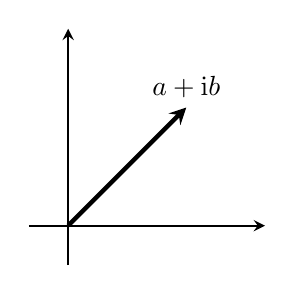
\begin{tikzpicture}[scale=0.5]
    \draw[-stealth,thick](-1,0)--(5,0);
    \draw[-stealth,thick](0,-1)--(0,5);
    \draw[-stealth,ultra thick](0,0)--(3,3);
    \coordinate[label=above:$a+\i b$] (z) at (3,3);
    \end{tikzpicture}
\end{center}
\begin{enumerate}[(1)]
    \item 模：$\abs{z}=r=\sqrt{a^2+b^2}$
\begin{property}

\end{property}
    \item 辐角：$\mathrm{Arg} z=\arg z\pm 2k\pi$，其主值为
    $$\arg z=\left\{
    \begin{aligned}
    &\arctan\frac{y}{x}&&\mbox{一、四象限}\\
    &\arctan\frac{y}{x}+\pi&&\mbox{二象限}\\
    &\arctan\frac{y}{x}-\pi&&\mbox{三象限}\\
    &\frac{\pi}{2}&&x=0,\ y>0\\
    &-\frac{\pi}{2}&&x=0,\ y<0\\
    &\pi&&x<0,\ y=0
    \end{aligned}
    \right.
    $$
\end{enumerate}
    \item 三角表示：$z=\abs{z}\left(\cos\theta+\i\sin\theta\right)$
    \item 极坐标：
    $\left\{
    \begin{aligned}
    &a=r\cos\theta\\
    &b=r\sin\theta
    \end{aligned}
    \right.
    $
    $$z=\abs{z}\left(\cos\theta+\i\sin\theta\right)$$
\item 指数表示
$$z=\abs{z}\mathrm{e}^{\i\theta}$$
Euler公式
    $$\mathrm{e}^{\i\theta}=\cos\theta+\i\sin\theta,\ \mathrm{e}^{\i\pi}+1=0$$
\end{enumerate}
\section{复数和复数的运算}
已知复数
$$z_1=a+\i b,\ z_2=c+\i d$$
\begin{enumerate}
    \item 加法减法
    $$z_1\pm z_2=\left(a\pm b\right)+\i\left(c\pm d\right)$$
    \item 乘法除法
    $$z_1z_2=\left(ac-bd\right)+\i\left(ad+bc\right)$$
    
    $$\frac{z_1}{z_2}=\frac{ac+bd}{c^2+d^2}+\i\frac{bc-ad}{c^2+d^2}$$
    其中$z_2\neq 0$
    \begin{property}
    模相乘，辐角相加
    $$z_1\cdot z_2\cdots z_n=\abs{z_1}\abs{z_2}\cdots\abs{z_n}\left[\cos\left(\theta_1+\theta_2+\cdots+\theta_n\right)+\i\sin\left(\theta_1+\theta_2+\cdots+\theta_n\right)\right]$$
    $$
    \left\{
    \begin{aligned}
    &z_1z_2=\abs{z_1}\abs{z_2}\mathrm{e}^{\i\left(\theta_1+\theta_2\right)}\\
    &\frac{z_1}{z_2}=\frac{\abs{z_1}}{\abs{z_2}}\mathrm{e}^{\i\left(\theta_1-\theta_2\right)}
    \end{aligned}
    \right.
    $$
    \end{property}
    \item 乘幂与方根\\
    若$z=\abs{z}\left(\cos\theta+\i\sin\theta\right)=\abs{z}\mathrm{e}^{\i\theta}$，则
    $$z^n=\abs{z}^n\left(\cos n\theta+\i\sin n\theta\right)=\abs{z}^n\mathrm{e}^{\i n\theta}$$
    $$\sqrt[n]{z}=\abs{z}^{\frac{1}{n}}\left(\cos\frac{\theta+2k\pi}{n}+\i\sin\frac{\theta+2k\pi}{n}\right)(k=0,1,2,\cdots,n-1)$$
\end{enumerate}
\subsection{复球面与无穷远点}
黎曼球：复平面上任意一点与球的北极点的连线和球面之间的交点表示复平面上的该点，则黎曼球的唯一确定的北极点代表复平面上多个方向的无穷远点.\\
\centerline{\includegraphics[width=9cm]{Riemann.jpg}}
\section{复变函数}
\begin{definition}
$w=f\left(z\right)$，在几何上可以看作把$z$平面上的一个点集$D$变到$w$平面上的一个点集$G$的映射.
$$
w=f\left(z\right)\left\{
\begin{aligned}
&u=u\left(x,y\right)\\
&v=v\left(x,y\right)
\end{aligned}
\right.
$$
即一个复变函数对应两个实变函数.
\end{definition}
\subsection{复变函数的极限}
设函数$f\left(z\right)=u\left(x,y\right)+\i v\left(x,y\right)$定义于$z_0=x_0+\i y$的去内邻域内，$A=u_0+\i v_0$，则$\lim_{z\to z_0}f\left(z\right)=A$的充要条件是
$$
\left\{
\begin{aligned}
&\lim_{\left(x,y\right)\to\left(x_0,y_0\right)}u\left(x,y\right)=u_0\\
&\lim_{\left(x,y\right)\to\left(x_0,y_0\right)}v\left(x,y\right)=v_0
\end{aligned}
\right.
$$
\chapter{解析函数}
\begin{definition}
\begin{enumerate}
    \item 极限：若对$\forall\varepsilon_0>0$，都$\exists\delta>0$，使得对$\forall x$，当$0<\abs{x-a}<\delta$时，都有$\abs{f\left(x\right)-A}<\varepsilon_0$，则称$A$为$f\left(x\right)$当$x$趋于$0$时的极限.
    \item 连续：当$\lim_{z\to a}f\left(z\right)=f\left(a\right)$时，称$f\left(z\right)$在$a$点连续.
    \item 导数：$f^{\prime}\left(z_0\right)=\lim_{\Delta z\to 0}\frac{f\left(z_0+\Delta z\right)-f\left(z_0\right)}{\Delta z}$
    \item 微分：若$w=f\left(z\right)$在$D$内可导，则$\dd w=f^{\prime}\left(z\right)\dd z$
\end{enumerate}
\end{definition}
\begin{definition}
\begin{enumerate}
    \item 点解析：$f\left(z\right)$在$z_0$及其$z_0$的邻域内可导，称$f\left(z\right)$在$z_0$点解析.
    \item 区域解析：$f\left(z\right)$在区域内每一点解析，称$f\left(z\right)$在区域内解析.
    \item 若$f\left(z\right)$在$z_0$点不解析，称$z_0$为$f\left(z\right)$的奇点.
\end{enumerate}
\end{definition}
\begin{theorem}
解析函数的运算法则：解析函数的和、差、积、商（除分母为零的点）仍为解析函数；解析函数的复合函数仍为解析函数.
\end{theorem}
\section{函数可导与解析的充要条件}
$f\left(z\right)=u\left(x,y\right)+\i v\left(x,y\right)$在$z=x+\i y$可导$\Longleftrightarrow u\left(x,y\right)$和$v\left(x,y\right)$在$D$内可导/可微，且满C-R条件：
$$
\left\{
\begin{aligned}
&\frac{\partial u}{\partial x}=\frac{\partial v}{\partial y}\\
&\frac{\partial u}{\partial y}=-\frac{\partial v}{\partial x}
\end{aligned}
\right.
$$
此时，$f^{\prime}\left(z\right)=\frac{\partial u}{\partial x}+\i\frac{\partial v}{\partial x}$
\begin{proof}
令
$$
\left\{
\begin{aligned}
&f\left(z\right)=u\left(z\right)+\i v\left(z\right)\\
&\Delta z=\Delta x+\i\Delta y
\end{aligned}
\right.
$$
则
$$
\begin{aligned}
\Delta f\left(z\right)&=f\left(z+\Delta z\right)-f\left(z\right)\\
&=\left[u\left(z+\Delta z\right)-u\left(z\right)\right]+\i\left[v\left(z+\Delta z\right)-v\left(z\right)\right]\\
&=\Delta u+i\Delta v
\end{aligned}
$$
$$f^{\prime}\left(z\right)=\lim_{\Delta z\to 0}\frac{\Delta f\left(z\right)}{\Delta z}=\lim_{\Delta z\to 0}\frac{\Delta u+\i\Delta v}{\Delta z}$$
得到沿$x$方向导数
$$f^{\prime}\left(z\right)=\lim_{\Delta x\to 0}=\lim_{\Delta x\to 0}\frac{\Delta u}{\Delta x}+\i\lim_{\Delta x\to 0}\frac{\Delta v}{\Delta x}=\frac{\partial u}{\partial x}+\i\frac{\partial v}{\partial y}$$
同理，沿$y$方向
$$f^{\prime}\left(z\right)=-\i\frac{\partial u}{\partial y}+\frac{\partial v}{\partial x}$$
要求两者相等，于是得到C-R条件
$$
\left\{
\begin{aligned}
&\frac{\partial u}{\partial x}=\frac{\partial v}{\partial y}\\
&\frac{\partial u}{\partial y}=-\frac{\partial v}{\partial x}
\end{aligned}
\right.
$$
\end{proof}
\section{复初等函数}
\begin{enumerate}
    \item 指数函数：$\mathrm{e}^z=\mathrm{e}^x\left(\cos y+\i\sin y\right)$，在$z$平面处处可导且解析，其周期为$2\pi\i$；$\left(\mathrm{e}^z\right)^{\prime}=\mathrm{e}^z$
    \item 对数函数：$\mathrm{Ln}z=\ln\abs{z}+\i\left(\arg z\pm 2k\pi\right)$为多值函数，其主值为$\ln z=\ln\abs{z}+\i\arg z$.$\mathrm{Ln}z$的每一个主值分支$\ln z$在除去原点及负实轴的$z$平面处处解析，且$\left(\ln z\right)^{\prime}=\frac{1}{z}$.
    \item 乘幂与幂函数：$z^b=\mathrm{e}^{b\mathrm{Ln}z}$
    \item 三角函数：$\sin z=\frac{\mathrm{e}^{\i z}-\mathrm{e}^{-\i z}}{2\i},\ \cos z=\frac{\mathrm{e}^{\i z}+\mathrm{e}^{-\i z}}{2},\ \tan z=\frac{\sin z}{\cos z}$，其中$\sin z$与$\cos z$在$z$平面内解析，且$\left(\sin z\right)^{\prime}=\cos z,\ \left(\cos z\right)^{\prime}=-\sin z$，二者有界性不再成立.
    \item 双曲函数：$\sinh z=\frac{\mathrm{e}^z-\mathrm{e}^{-z}}{2},\ \cosh z=\frac{\mathrm{e}^z+\mathrm{e}^{-z}}{2}$，其中$\left(\sinh z\right)^{\prime}=\cosh z,\ \left(\cosh z\right)^{\prime}=\sinh z$
\end{enumerate}
\chapter{复变函数的积分}
\section{复变函数积分的概念与性质}
\begin{definition}
$$\int_c{f\left(z\right)\dd z=\lim_{n\to\infty}}\sum_{k=1}^n{f\left(\xi_k\right)\Delta z_k}$$
为复变函数积分，即复平面上的线积分，其中$c$是光滑曲线.
\end{definition}
\subsection{复变函数积分计算方法}
\begin{enumerate}
    \item 化为线积分：$\int_c{f\left(z\right)\dd z}=\int_c{u\dd x-v\dd y}+\i\int_c{v\dd x+u\dd y}$
    \item 参数方法：设曲线$c:z=z\left(t\right)(\alpha\leq t\leq\beta)$，其中$\alpha,\ \beta$分别对应曲线的起点、终点，则$\int_c{f\left(z\right)\dd z}=\int_{\alpha}^{\beta}{f\left[z\left(t\right)\right]z^{\prime}\left(t\right)\dd t}$
\end{enumerate}
\begin{theorem}
\begin{enumerate}
    \item 柯西-古萨定理：设$f\left(z\right)$在单连通区域$B$内解析，$c$为$B$内任一闭曲线，则$\int_c{f\left(z\right)\dd z}=0$
    \item 复闭合回路定理：设$f\left(z\right)$在多连通区域$D$内解析，$c$为$D$内任意一条简单闭曲线，$c_1,\ c_2,\cdots,\ c_n$是$c$内的简单闭曲线，它们互不包含互不相交，并且以$c_1,\ c_2,\cdots,\ c_n$是$c$为边界的区域全含于$D$内，则
    $$\int_c{f\left(z\right)\dd z}=\sum_{k=1}^{n}{\int_{c_k}{f\left(z\right)\dd z}},\ \int_{\Gamma}{f\left(z\right)\dd z}=0$$
    其中$\Gamma$由$c$及$c^{-1}$（$k=1,2,\cdots,n$）所组成的复合闭路.
    $$
    \oint_c{\frac{1}{\left(z-z_0\right)^{n+1}}\dd z}=
    \left\{
    \begin{aligned}
    &2\pi\i&&n=0\\
    &0&&n\neq 0
    \end{aligned}
    \right.c\mbox{为包含}z_0\mbox{的正向闭曲线}
    $$
\end{enumerate}
\end{theorem}
\subsection{柯西积分公式与高阶导数公式}
\begin{enumerate}
    \item 柯西积分公式：$f$在$D$内处处解析，$C$为$D$内正向闭曲线，$z_0$为$c$内部一点，则有
    $$f\left(z_0\right)=\frac{1}{2\pi\i}\oint_L{\frac{f\left(z\right)}{z-z_0}\dd z}$$
    \item 高阶导数公式：解析函数$f$的导数仍为解析函数
    $$f^{\left(n\right)}\left(z_0\right)=\frac{n!}{2\pi\i}\oint_c{\frac{f\left(\xi\right)}{\left(\xi-z_0\right)^{n+1}}\dd\xi}$$
    \item 柯西不等式：设$f$在$D$内解析，$z_0\in D$，圆周$K_R=\left\{z\bigg|\abs{z-z_0}=R\right\}$及其内部均含于$D$，则
    $$\abs{f^{\left(n\right)}\left(z_0\right)}\leq\frac{n!M\left(R\right)}{R^n}$$
    \item 刘维尔定理：若$f\left(z\right)$在整个复平面上解析且有界，则$f\left(z\right)$在复平面上恒为常数.
    \item 莫雷拉定理：若$f\left(z\right)$在单连通$B$内连续，且对$B$内任一闭曲线$c$都有$\oint_c{f\left(z\right)\dd z}=0$，则$f$在$B$解析.
\end{enumerate}
\subsection{解析函数与调和函数的关系}
已知二元实函数$\varphi\left(x,y\right)$满足$\frac{\partial^2\varphi}{\partial x^2}+\frac{\partial^2\varphi}{\partial y^2}=0$，其中$\varphi$为调和函数：
\begin{theorem}
\begin{enumerate}
    \item 若$f\left(z\right)=u\left(x,y\right)+\i v\left(x,y\right)$在区域$D$内解析，则$u,\ v$都是$D$内的调和函数，即
    $$u_{xx}+u_{yy}=0,\ v_{xx}+v_{yy}=0$$
    \item 设$u\left(x\right)$为$D$内调和函数，若$D$内另一个函数$v\left(x,y\right)$使$u+\i v$在$D$内构成解析函数，则$v$为$u$的共轭调和函数，即:若$u$与$v$在$D$内满足C-R方程，则$v$为$u$的共轭调和函数.
\end{enumerate}
\end{theorem}
\chapter{复变函数的级数}
\section{复数项级数}
    \begin{theorem}
    复数列$\left\{\alpha_n\right\}=\left\{a_n+\i b_n\right\}(n=1,2,\cdots)$收敛于复数$\alpha=a+\i b$的充要条件为
    $$\lim_{n\to\infty}a_n=a,\ \lim_{n\to\infty}b_n=b$$
    即复数列$\left\{\alpha_n\right\}$收敛$\Longleftrightarrow$实数列$\left\{a_n\right\},\ \left\{b_n\right\}$同时收敛.
    \begin{enumerate}
        \item 复数项级数$\sum_{n=0}^{\infty}{\alpha_n}$收敛的充要条件是级数$\sum_{n=0}^{\infty}{a_n}$与级数$\sum_{n=0}^{\infty}{b_n}$同时收敛.
        \item 级数收敛的必要条件是$\lim_{n\to\infty}\alpha_n=0$
        \item $\sum_{n=1}^{\infty}{\abs{\alpha_n}}$收敛，则$\sum_{n=1}^{\infty}\alpha_n$收敛，且$\abs{\sum_{n=1}^{\infty}{\alpha_n}}\leq\sum_{n=1}^{\infty}{\abs{\alpha_n}}$
        \item $\sum_{n=1}^{\infty}{\alpha_n}$绝对收敛$\Longleftrightarrow\sum_{n=1}^{\infty}{a_n}$与$\sum_{n=1}^{\infty}{b_n}$绝对收敛
    \end{enumerate}
    \end{theorem}

\section{幂级数的敛散性}
\begin{definition}
幂级数：表达式$\sum_{n=0}^{\infty}{c_n\left(z-z_0\right)^n}$或$\sum_{n=0}^{\infty}{c_nz^n}$为幂级数.
\end{definition}
\begin{theorem}
Abel定理（幂级数的收敛定理）：如果幂级数$\sum_{n=0}^{\infty}{c_nz^n}$在$z_0\neq 0$处收敛，那么对满足$\abs{z}<\abs{z_0}$的一切$z$，级数绝对收敛；如果在$z_0$处发散，那么对满足$\abs{z}>\abs{z_0}$的一切$z$，级数必发散.
\end{theorem}
\subsection{收敛半径}
$$\lim_{n\to\infty}\abs{\frac{c_{n+1}}{c_n}}=\lambda=\frac{1}{R},\ \lim_{n\to\infty}\sqrt[n]{\abs{c_n}}=\lambda=\frac{1}{R}$$
\begin{enumerate}
    \item 有理运算后，在$\abs{z}<\min\left\{r_1,r_2\right\}$内依旧收敛.
    \item 级数$\left(\sum_{n=0}^{\infty}a_nz^n\right)\left(\sum_{n=0}^{\infty}b_nz^n\right)$在$D$内收敛，则$f\left(z\right)g\left(z\right)=\left(\sum_{n=0}^{\infty}a_nz^n\right)\left(\sum_{n=0}^{\infty}b_nz^n\right)=\sum_{n=0}^{\infty}{c_nz}$
\end{enumerate}
\begin{property}
若$f\left(z\right)=\sum_{n=0}^{\infty}{c_n\left(z-a\right)^n}$，则
\begin{enumerate}
    \item $f\left(z\right)$是收敛圆$\abs{z-a}=R$内的解析函数
    \item $f\left(z\right)$在收敛圆内任意阶可导，并且可以逐项求导
    $$f^{\left(n\right)}\left(z\right)=\left(\sum_{n=0}^{\infty}{c_n\left(z-a\right)^n}\right)^{\left(k\right)}=\sum_{n=0}^{\infty}{\left[c_n\left(z-a\right)^n\right]^{\left(k\right)}}$$
    \item $f\left(z\right)$在收敛圆内可积，并且可以逐项积分
    $$\int_c{f\left(z\right)\dd z}=\sum_{n=0}^{\infty}{c_n\int_c{\left(z-a\right)^n\dd z}}$$
\end{enumerate}
\end{property}
\section{泰勒级数}
\begin{theorem}
$f\left(z\right)$在圆域$k=\left\{z\bigg|\abs{z-z_0}<R\right\}$内解析，则在$k$内$f\left(z\right)$能唯一地展开成
$$f\left(z\right)=\sum_{n=0}^{\infty}{c_n\left(z-z_0\right)^n}$$
其中，$c_n=\frac{1}{2\pi\i}\oint_c\frac{f\left(\xi\right)}{\left(\xi-z_0\right)^{n-1}\dd\xi}=\frac{f^n\left(z_0\right)}{n!},\ c=\left\{\xi\bigg|\abs{\xi-z_0}=\rho\right\}$
\end{theorem}
\begin{corollary}
设函数在区域$D$内解析，$z_0\in D$，$\alpha$为$f\left(z\right)$在$D$内距$z_0$最近的一个奇点，则使展开式$f\left(z\right)=\sum_{n=0}^{\infty}{c_n\left(z-z_0\right)^n}$成立的半径$R=\abs{\alpha-z_0}$
\begin{property}
幂级数的收敛性与其和函数的解析性无必然关系，即使幂级数在其收敛圆上处处收敛，其和函数在收敛圆上仍然至少有一个奇点.
\end{property}
\begin{note}
$f$在$D$内解析$\Longleftrightarrow f$在$D$内任一点的邻域内可以展开成$z-z_0$的幂级数.
\end{note}
\end{corollary}
\section{洛朗级数}
\begin{definition}
收敛圆环域：以$z_0$为中心的某一圆环域中
$$\sum_{n=-\infty}^{\infty}{c_n\left(z-z_0\right)^n}=\sum_{n=1}^{+\infty}{c_{-n}\left(z-z_0\right)^{-n}}+\sum_{n=0}^{+\infty}{c_n\left(z-z_0\right)^n}$$
其中，$\sum_{n=1}^{+\infty}{c_{-n}\left(z-z_0\right)^{-n}}$在$\abs{z-z_0}>R_1$内收敛，$\sum_{n=0}^{+\infty}{c_n\left(z-z_0\right)^n}$在$\abs{z-z_0<R_2}$内收敛，则其收敛圆域为$R_1<\abs{z-z_0}<R_2$
\begin{property}
和函数解析、可逐项积分、可逐项求导.
\end{property}
\end{definition}
\chapter{孤立奇点与留数定理}
\section{孤立奇点的概念与分类}
\begin{definition}
孤立奇点：函数$f\left(z\right)$在$z_0$点不解析，但在$z_0$的$0<\abs{z-z_0}<\delta$内解析.
\end{definition}
\section{孤立奇点的类型}
\begin{enumerate}
    \item 可去奇点：展开式中不含$z-z_0$的负幂项：$f\left(z\right)=c_0+c_1\left(z-z_0\right)+c_2\left(z-z_0\right)^2+\cdots$
    \item 极点：展开式中含有限项$z-z_0$的负幂项
    $$f\left(z\right)=\frac{c_{-m}}{\left(z-z_0\right)^{m}}+\frac{c_{-\left(m-1\right)}}{\left(z-z_0\right)^{m-1}}+\cdots+\frac{c_{-1}}{\left(z-z_0\right)}+c_0+c_1\left(z-z_0\right)+c_2\left(z-z_0\right)^2+\cdots=\frac{g\left(z\right)}{\left(z-z_0\right)^m}$$
    其中$g\left(z\right)=c_{-m}+c_{-\left(m-1\right)}\left(z-z_0\right)+\cdots+c_{-1}\left(z-z_0\right)^{m-1}+c_0\left(z-z_0\right)^m+\cdots$在$z_0$解析，且$g\left(z_0\right)\neq 0,\ m\geq 1,\ c_{-m}\neq 0$
    \item 本性奇点：展开式中含无穷多项$z-z_0$的负幂项
    $$f\left(z\right)=\cdots+\frac{c_{-m}}{\left(z-z_0\right)^m}+\cdots+\frac{c_{-1}}{\left(z-z_0\right)}+c_0+c_1\left(z-z_0\right)+\cdots+c_m\left(z-z_0\right)^m+\cdots$$
\end{enumerate}
\section{孤立奇点的判别方法}
\begin{enumerate}
    \item 可去奇点：$\lim_{z\to z_0}f\left(z\right)=c_0$
    \item 极点：$\lim_{z\to z_0}f\left(z\right)=\infty$
    \item 本性奇点：$\lim_{z\to z_0}f\left(z\right)$不存在且不为$\infty$
    \item 零点与极点的关系：$z_0$是$f\left(z\right)$的$m$级零点$\Longleftrightarrow z_0$是$\frac{1}{f\left(z\right)}$的$m$级极点；
    \begin{definition}
    零点：不恒为零的解析函数$f\left(z\right)$，如果能表示成$f\left(z\right)=\left(z-z_0\right)^m\varphi\left(z\right)$，其中$\varphi\left(z\right)$在$z_0$解析，$\varphi\left(z_0\right)\neq 0,\ m$为正整数，称$z_0$为$f\left(z\right)$的$m$级零点
    \end{definition}
    \begin{theorem}
    零点级数判别的充要条件\\
    $z_0$是$f\left(z\right)$的$m$级零点$\Longleftrightarrow
    \left\{
    \begin{aligned}
    &f^{\left(n\right)}\left(z_0\right)=0\\
    &f^{\left(m\right)}\left(z_0\right)\neq 0
    \end{aligned}
    \right.(n=1,2,\cdots,m-1)
    $
    \end{theorem}
\end{enumerate}
\section{留数的基本概念}
\begin{definition}
设$z_0$为$f\left(z\right)$的孤立奇点，$f\left(z\right)$在去心邻域$0<\abs{z-z_0}<\delta$内解析，$c$为该域内包含$z_0$的任一正向简单闭曲线，则称积分$\frac{1}{2\pi\i}\int_c{f\left(z\right)\dd z}$为$f\left(z\right)$在$z_0$的留数，记作$\Res\left[f\left(z\right),z_0\right]=\frac{1}{2\pi\i}\int_c{f\left(z\right)\dd z}$
\end{definition}
\subsection{留数的计算方法}
\begin{enumerate}
    \item 可去奇点处的留数
    \begin{theorem}
    若$z_0$是$f\left(z\right)$的可去极点，则$\Res\left[f\left(z\right),z_0\right]=0$
    \end{theorem}
    \item $m$级极点处的留数
    \begin{theorem}
    \begin{enumerate}
        \item 若$z_0$是$f\left(z\right)$的一级极点，则$\Res\left[f\left(z\right),z_0\right]=\lim_{z\to z_0}\left(z-z_0\right)f\left(z\right)$
        \item 若$z_0$是$f\left(z\right)$的$m$级极点，则$\Res\left[f\left(z\right),z_0\right]=\frac{1}{\left(m-1\right)!}\lim_{z\to z_0}\frac{\dd^{m-1}}{\dd z^{m-1}}\left[\left(z-z_0\right)^mf\left(z\right)\right]$，若级数小于$m$，依旧看作级数等于$m$进行计算.
    \end{enumerate}
    \end{theorem}
    \item 设$f\left(z\right)=\frac{P\left(z\right)}{Q\left(z\right)}$，$P\left(z\right),\ Q\left(z\right)$在$z_0$解析，$P\left(z_0\right)\neq 0,\ Q\left(z_0\right)=0,\ Q^{\prime}\left(z_0\right)\neq 0$，则$\Res\left[\frac{P\left(z\right)}{Q\left(z\right)},z_0\right]=\frac{P\left(z\right)}{Q^{\prime}\left(z\right)}$
    \item 无穷远点的留数：$\Res\left[f\left(z\right),\infty\right]=\frac{1}{2\pi\i}\int_{c^-}{f\left(z\right)\dd z}=-c_{-1}$
\end{enumerate}
\section{留数基本定理}
\begin{theorem}
设$f\left(z\right)$在区域$D$内除有限个孤立奇点$z_1,\ z_2,\ \cdots,\ z_n$外处处解析，$c$为$D$内包围所有奇点的一条正向简单闭曲线，则$\int_c{f\left(z\right)\dd z}=2\pi\i\sum_{n=1}^{\infty}{\Res\left[f\left(z\right),z_n\right]}$
\end{theorem}
\section{留数定理在计算实积分上的应用}
\begin{example}
形如$\int_0^{2\pi}{R\left(\cos\theta,\i\sin\theta\right)\dd\theta}$的积分
    $$\int_0^{2\pi}{R\left(\cos\theta,\sin\theta\right)\dd\theta}=\oint_{\abs{z}=1}{R\left(\frac{z+z^{-1}}{2},\frac{z-z^{-1}}{2\i}\right)\frac{\dd z}{\i z}}=\oint_{\abs{z=1}}{f\left(z\right)\dd z}$$
    则$\int_0^{2\pi}{R\left(\cos\theta,\sin\theta\right)\dd\theta}=2\pi\i\sum_{k=1}^n{\Res\left[f\left(z\right),z_k\right]}$，其中$z_k$为$\abs{z}=1$内的奇点；若$R\left(\cos\theta,\sin\theta\right)$为$\theta$的偶函数，则也可用$z=\mathrm{e}^{\i\theta}$来计算.
\end{example}
\begin{example}
形如$\int_{-\infty}^{+\infty}{R\left(x\right)\dd x}$的积分（其中$R\left(x\right)=\frac{P_m\left(x\right)}{Q_m\left(x\right)}=\frac{a_0+a_1x+\cdots+a_mx^m}{b_0+b_1x+\cdots+b_nx^n}$，$a_m\neq 0,\ b_n\neq 0,\ n-m\geq 2$，$R\left(z\right)$在实轴上无奇点），则
    $$\int_{-\infty}^{+\infty}{R\left(x\right)\dd x}=2\pi\i\sum_{k=1}^n{\Res\left[R\left(z\right),z_k\right]}$$
    其中$z_k$为上半平面所有奇点；若$R\left(x\right)$为偶函数，则$\int_0^{+\infty}{R\left(x\right)\dd x}=\pi\i\sum_{k=1}^n{\Res\left[R\left(z\right),z_k\right]}$
\end{example}
\begin{example}
形如$\int_{-\infty}^{+\infty}{R\left(x\right)\mathrm{e}^{\i ax}\dd x}(a>0)$的积分（$n-m\geq 1$，$R\left(z\right)$在实轴上无奇点），则
    $$
    \begin{aligned}
    \int_{-\infty}^{+\infty}{R\left(x\right)\mathrm{e}^{\i ax}\dd x}&=2\pi\i\sum_{k=1}^n{\Res\left[R\left(z\right)\mathrm{e}^{\i az},z_k\right]}\\
    &=\int_{-\infty}^{+\infty}{R\left(x\right)\cos ax\dd x}+\i\int_{-\infty}^{+\infty}{R\left(x\right)\sin ax\dd x}\\
    &=\Re\left(2\pi\i\sum\Res\left[R\left(z\right)\mathrm{e}^{\i az},z_k\right]\right)+\Im\left(2\pi\i\sum\Res\left[R\left(z\right)\mathrm{e}^{\i az},z_k\right]\right)
    \end{aligned}
    $$
\end{example}
\end{spacing}
\end{document}